\section{Dispatcher module}
\label{sec:Dispatcher}
\subsection{Introduction}
In order to distribute the load in several machines, this module is responsible to assign a demorunner according to a policy and the given requirements. 
The demorunners list is provided by the core module wich is in charge of reading the demorunners.xml where all the demorunners are. If the 
demorunner.xml file changes, there are two ways for reload the list loaded in memory, the first one is calling the function refresh\_demorunners
in the core and the other one is reloading the core and dispatcher module.

Figure \ref{fig:core_diagram} shows a diagram that explains the modules and the messages passed when executing an experiment. 
%
\begin{figure}[!ht]
\centering
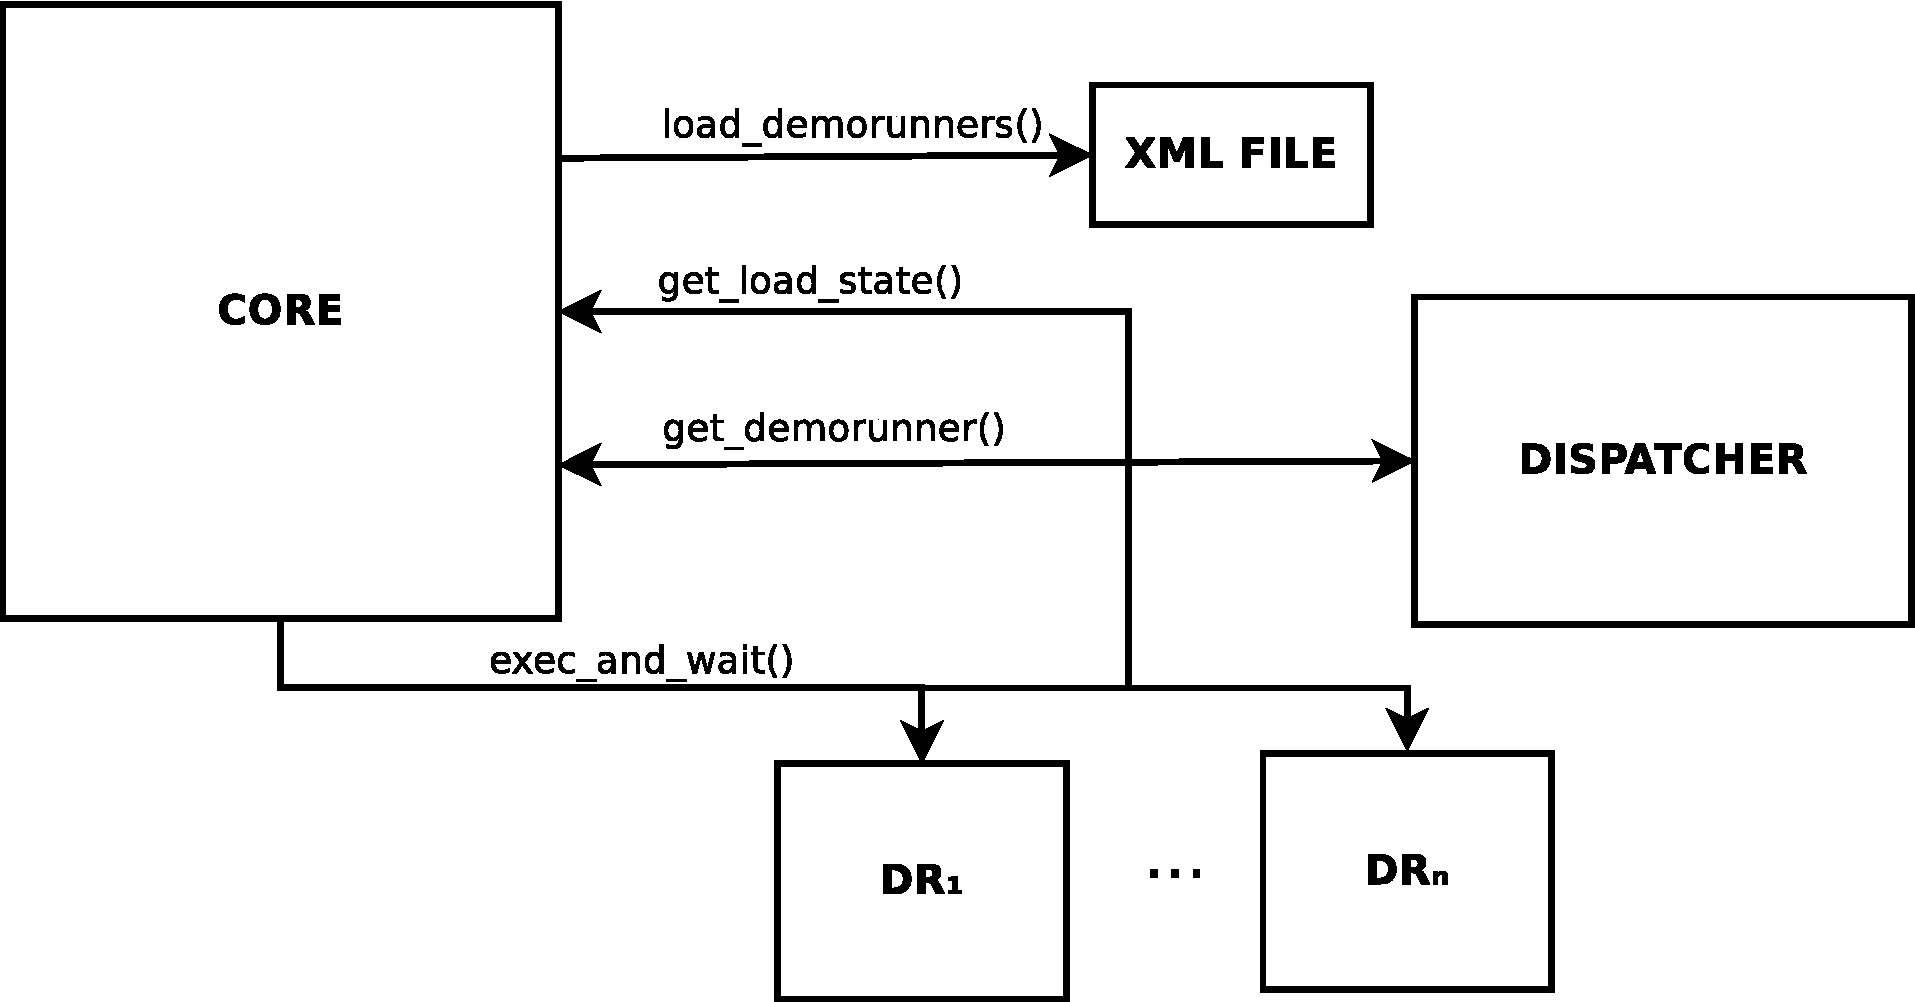
\includegraphics[width=0.7\columnwidth]{dispatcher/images/core_dispatcher.pdf}
\caption{Communication between the Core, Dispatcher, and the DemoRunner modules.}
\label{fig:core_diagram}
\end{figure}

\subsection{Policies}
The creation of the policies are made by the Factory Method, allowing the implementation and assignment of new policies in an easy way.
Until now the implemented policies are:

\begin{itemize}
\item \textbf{Random Policy:} this policy assigns a random demorunner from the available demorunners list that matches the requirements.
\item \textbf{Sequential Policy:} this policy iterates from the available demorunners list that matches the requirements.
\item \textbf{Lowest Workload Policy:} this policy assigns the demorunner with the lowest workload from the available demorunners list that matches the requirements.
\end{itemize}


